
\documentclass[final]{beamer}

\usepackage[scale=1.24, orientation=portrait]{beamerposter} % Use the beamerposter package for laying out the poster

\usetheme{confposter} % Use the confposter theme supplied with this template

%\setbeamercolor{block title}{fg=ngreen,bg=white} % Colors of the block titles
%\setbeamercolor{block body}{fg=black,bg=white} % Colors of the body of blocks
%\setbeamercolor{block alerted title}{fg=white,bg=dblue!70} % Colors of the highlighted block titles
%\setbeamercolor{block alerted body}{fg=black,bg=dblue!10} % Colors of the body of highlighted blocks
\setbeamercolor{block alerted title}{fg=dgreen,bg=white} % Change the alert block title color
\setbeamercolor{block alerted body}{fg=black,bg=white} % Change the alert block body colors
\setbeamercolor{block title}{fg=dblue,bg=white} % Change the block title color
% Many more colors are available for use in beamerthemeconfposter.sty

%-----------------------------------------------------------
% Define the column widths and overall poster size
% To set effective sepwid, onecolwid and twocolwid values, first choose how many columns you want and how much separation you want between columns
% In this template, the separation width chosen is 0.024 of the paper width and a 4-column layout
% onecolwid should therefore be (1-(# of columns+1)*sepwid)/# of columns e.g. (1-(4+1)*0.024)/4 = 0.22
% Set twocolwid to be (2*onecolwid)+sepwid = 0.464
% Set threecolwid to be (3*onecolwid)+2*sepwid = 0.708

\newlength{\sepwid}
\newlength{\onecolwid}
\newlength{\twocolwid}
\newlength{\threecolwid}
\setlength{\paperwidth}{36in}
\setlength{\paperheight}{48in} 
\setlength{\sepwid}{0.08\paperwidth} % Separation width (white space) between columns
\setlength{\onecolwid}{0.38\paperwidth} % Width of one column
\setlength{\twocolwid}{0.76\paperwidth} % Width of two columns
%\setlength{\threecolwid}{0.708\paperwidth} % Width of three columns
\setlength{\topmargin}{-0.5in} % Reduce the top margin size


%-----------------------------------------------------------

\usepackage{graphicx}  % Required for including images

\usepackage{booktabs} % Top and bottom rules for tables

%----------------------------------------------------------------------------------------
%	TITLE SECTION 
%----------------------------------------------------------------------------------------

\title{Semi-supervised classification \\by reaching consensus among modalities} % Poster title

\author{Zining Zhu$^{1,2,5}$, Jekaterina Novikova$^1$, Frank Rudzicz$^{3,5,2,4,1}$} % Author(s)

\institute{$^1$Winterlight Labs, $^2$University of Toronto, $^3$Li Ka Shing Knowledge Institute, St Michael's Hospital, Toronto ON\\$^4$Surgical Safety Technologies, $^5$Vector Institute} % Institution(s)

%----------------------------------------------------------------------------------------

\begin{document}

\addtobeamertemplate{block end}{}{\vspace*{2ex}} % White space under blocks
\addtobeamertemplate{block alerted end}{}{\vspace*{2ex}} % White space under highlighted (alert) blocks

\setlength{\belowcaptionskip}{2ex} % White space under figures
\setlength\belowdisplayshortskip{2ex} % White space under equations

\begin{frame}[t] % The whole poster is enclosed in one beamer frame

\begin{columns}[t] % The whole poster consists of three major columns, the second of which is split into two columns twice - the [t] option aligns each column's content to the top

\begin{column}{\sepwid}\end{column} % Empty spacer column

\begin{column}{\onecolwid} % The first column

%----------------------------------------------------------------------------------------
%	OBJECTIVES
%----------------------------------------------------------------------------------------

\begin{alertblock}{Summary}
\begin{itemize}
\item We present \textbf{Transductive Consensus Networks} (TCN), extending Consensus Networks into semi-supervised learning.
\item Analyze its two meahcnisms: consensus and classification, with ablation studies.
\item Quantify agreement with similarity: negative relative JSD.
\item Show that good classification require imperfect consensus.
\end{itemize}

\end{alertblock}

%----------------------------------------------------------------------------------------
%	QUICK REVISION
%----------------------------------------------------------------------------------------

\begin{block}{Background}
\textbf{Problem Setting}
\begin{itemize}
    \item Training data and reliable labels can be expensive to acquire.
    \item For the available data, features from multiple views are available.
\end{itemize}

\textbf{Previous solutions}
\begin{itemize}
    \item \textbf{Multi-view learning}: Co-train, tri-train, Consensus Network.
    \item \textbf{Semi-supervised learning}: Ladder, CatGAN, TSVM.
\end{itemize}

Consensus Network (CN)\cite{CN2018} is useful for multi-modal learning. We extend CN to Transductive Consensus Networks (TCN).

\end{block}

\begin{block}{From CN to TCN}
\begin{figure}
    \centering
    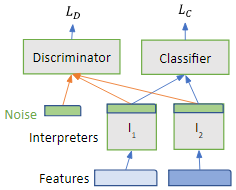
\includegraphics[width=.6\textwidth]{images/TCN_model.png}
    \caption{CN \& TCN with M=2 modalities. (Sections 3.2 - 3.3 in paper)}
    \label{fig:cn_structure}
\end{figure}

\begin{itemize}
    \item \textbf{Interpreters} $I_m$ compress modal features into representations.
    %\[\mathbf{v_m} = I_m(\mathbf{x_m})\] 
    
    \item \textbf{Discriminator} $D$ tries to tell their originating modalities. 
    %\[ D(\mathbf{v_m}) = P(\mathbf{x_m} \in \mathcal{M}_m|I_{1..M},D) \] 
    
    \item Inject `noise modality' to enhance discriminator ability
    %\[ \mathbf{v_{M+1}} \sim \mathcal{N}(\mathbf{\mu_{v_{1..M}}, \mathbf{\sigma^2_{v_{1..M}}}}) \]
    
    \item \textbf{Classifier} $C$ makes predictions from combined representations
    %\[ C([\mathbf{v_1}, \mathbf{v_2}, ..., \mathbf{v_M}]) = P(y | \mathbf{x}, I_{1..M}, C)  \] 
\end{itemize}

\textbf{Training the model} (Section 3.3 in paper)
\begin{itemize}
    \item Set up cross-entropy losses for discriminator $\mathcal{L_D}$ and classifier $\mathcal{L_C}$.
    \item Mechanisms: Consensus $\displaystyle \max_{I_{1..M}}\min_{D} \mathcal{L_D}$; Classification $\displaystyle \min_{I_{1..M}, C} \mathcal{L_C}$.
    %\item GAN-style iterative training.
    \item In CN, all training data are labeled.
    \item In TCN, only classification mechanism use labeled data. The consensus mechanism \textbf{uses non-labeled data}.
\end{itemize}

\end{block}

\begin{block}{Reference}
\bibliographystyle{unsrt}
\bibliography{bibliography}
\end{block}


\end{column} % End of the first column

\begin{column}{\sepwid}\end{column} % Empty spacer column


\begin{column}{\onecolwid} % The second column

\begin{block}{Ablation studies on mechanisms}
We implement three TCN variants as ablation studies on the two mechanisms. (Section 3.4 in paper)
\begin{itemize}
    \item TCN-embed: emphasize consensus mechanism.
    \item TCN-SVM: remove classifier mechanism. Use SVM instead.
    \item TCN-AE: inhibit consensus mechanism with autoencoders.
\end{itemize}
\end{block}

\begin{figure}[h]
    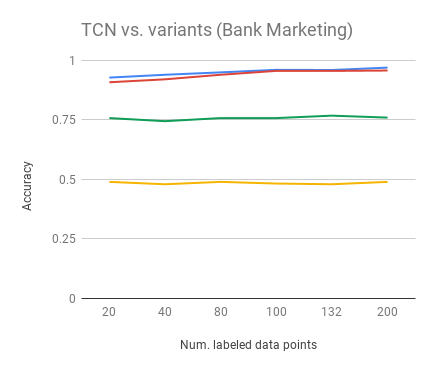
\includegraphics[width=.42\textwidth]{images/accuracy_variants_bm.png}
    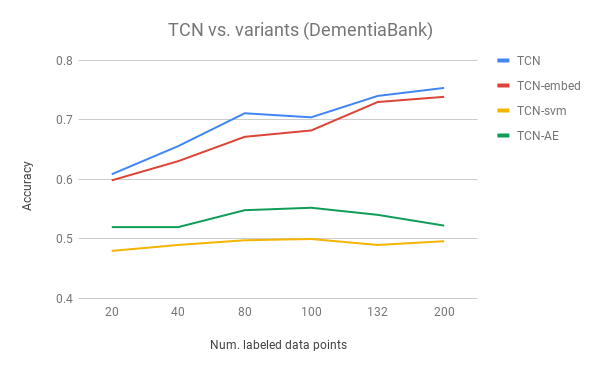
\includegraphics[width=.58\textwidth]{images/accuracy_variants_db.png}
    \caption{Accuracy plots for TCN vs its variants. TCN-embed accuracies aligns with TCN, both significantly outperforming TCN-AE, which is better than TCN-svm. The consensus and classification mechanisms should both be present.}
    \label{fig:accuracy_tcn_vs_variants}
\end{figure}


\begin{block}{Similarity of representations}
We measure similarity of representations with the negative relative JS divergence: (Section 3.5 in paper)
\[\hat{D}(p_m || p_n) = \frac{1}{2(\mathbb{H}_{p_m} +  \mathbb{H}_{p_n})} (D_{KL}(p_m || p_n) + D_{KL}(p_n || p_m))\]
\[ \displaystyle \text{Similarity} = \mathbb{E}_i \mathbb{E}_{m,n\in \{1..M\} \text{ and } m\neq n} \big \{-\hat{D}(p_m^{(i)} || p_n^{(i)}) \big \} \]

\begin{figure}
    \centering
    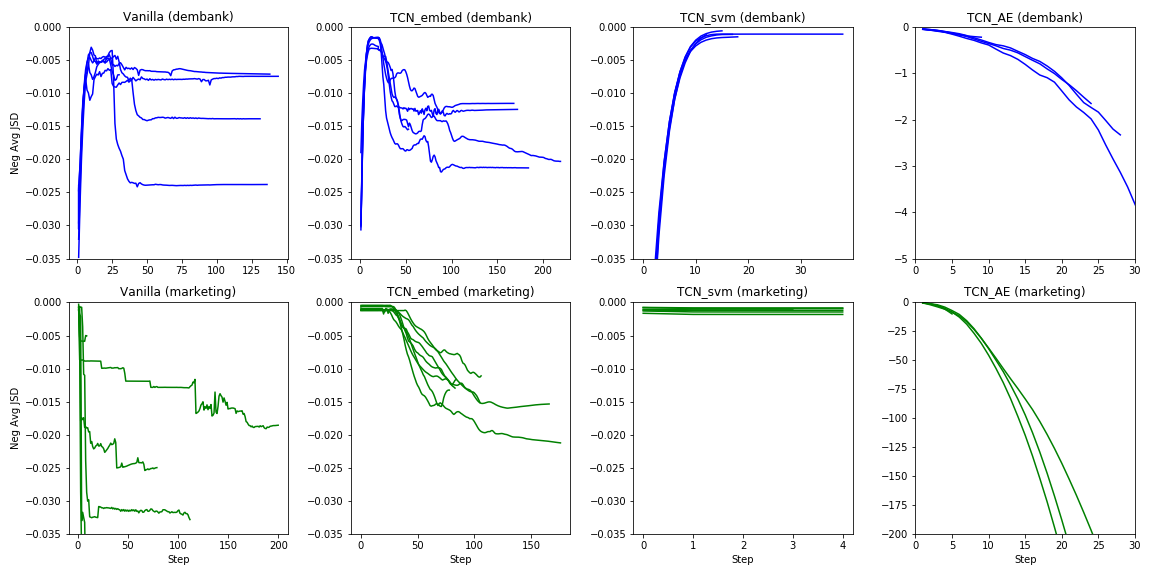
\includegraphics[width=.9\textwidth]{images/tcn_collective_rmi.png}
    \caption{Similarity plots on DementiaBank with 80 labels (blue) and Bank Marketing with 20 (green), for TCN and its three variants.}
    \label{fig:my_label}
\end{figure}
\end{block}


\begin{block}{Accuracy versus benchmarks}
\begin{figure}[h]
    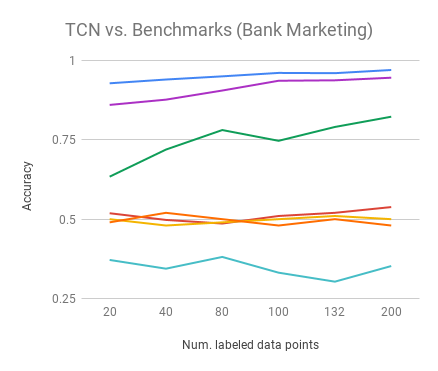
\includegraphics[width=.42\textwidth]{images/accuracy_plot_bm.png}
    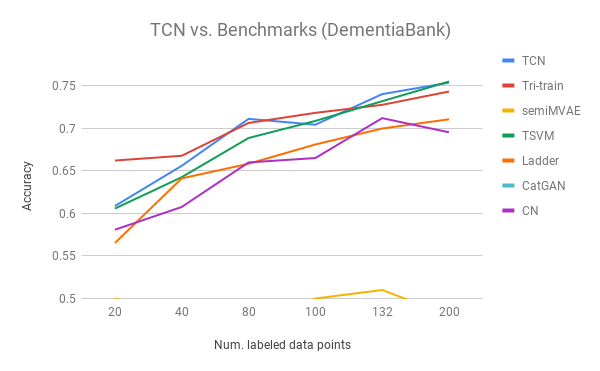
\includegraphics[width=.58\textwidth]{images/accuracy_plot_db.png}
    \caption{TCN (top blue lines) outperform or align with benchmark algorithms, including multi-modal semi-supervised (tri-train, uni-modal semi-supervised (TSVM, Ladder, CatGAN, and multi-modal supervised (CN). (Section 4 - 5 in paper.)}
    \label{fig:accuracy_tcn_vs_benchmarks}
\end{figure}
\end{block}


%----------------------------------------------------------------------------------------
%	ACKNOWLEDGEMENTS
%----------------------------------------------------------------------------------------


%\begin{block}{References}
%\bibliographystyle{plain}
%\bibliography{sample}
%\end{block}


%----------------------------------------------------------------------------------------

\end{column} % End of the second column

\end{columns} % End of all the columns in the poster

\end{frame} % End of the enclosing frame

\end{document}





\iffalse
%\setbeamercolor{block title}{fg=red,bg=white} % Change the block title color

\setbeamercolor{block alerted title}{fg=black,bg=norange} % Change the alert block title colors
\setbeamercolor{block alerted body}{fg=black,bg=white} % Change the alert block body colors

\begin{alertblock}{Some Necessary and Useful Vocabulary}

\begin{itemize}
\item (n.) sign $\rightarrow$ $+$ or $-$
\item (n.) equation $\rightarrow something = 0$ 
\item (n.) factor $\rightarrow$ two multiplied factors give result
\item (v.) factorise $\rightarrow$ putting into brackets
\item (n.) coefficient $\rightarrow$ a constant number i.e. $a$, $b$, $c$ in a pattern $ax^2+bx+c$
\item (n.) quadratic function $\rightarrow$ $f(x) = ax^2+bx+c$
\item (n.) root $\rightarrow$ $\sqrt{sth}$ or solution of quadratic equation
\item (n.) formula $=$ pattern
\end{itemize}

\end{alertblock}
\fi